% !TeX root = ./handout-09.tex

\setcounter{section}{8}

\section{Identity}
\subsection{The identity predicate}

\begin{frame}
  \frametitle{Greta admires everyone (else)}

\usetikzlibrary{arrows}
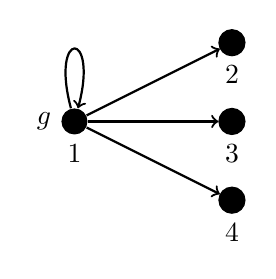
\begin{tikzpicture}
    \node[circle,fill,label={below:$1$},label={left:$g$}] (A) at (-1,0) {};
    \node[circle,fill,draw,label={below:$2$}] (B) at (1,1) {};
    \node[circle,fill,draw,label={below:$3$}] (C) at (1,0) {};
    \node[circle,fill,draw,label={below:$4$}] (D) at (1,-1) {};
    \draw[->,thick] (A) to[loop above,looseness=30] (A);
    \draw[->,thick] (A) -- (B);
    \draw[->,thick] (A) -- (C);
    \draw[->,thick] (A) -- (D);
\end{tikzpicture}
\hfill
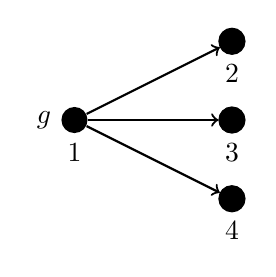
\begin{tikzpicture}
  \node[circle,fill,label={below:$1$},label={left:$g$}] (A) at (-1,0) {};
  \node[circle,fill,draw,label={below:$2$}] (B) at (1,1) {};
  \node[circle,fill,draw,label={below:$3$}] (C) at (1,0) {};
  \node[circle,fill,draw,label={below:$4$}] (D) at (1,-1) {};
  %\draw[->,thick] (A) to[loop above,looseness=30] (A);
  \draw[->,thick] (A) -- (B);
  \draw[->,thick] (A) -- (C);
  \draw[->,thick] (A) -- (D);
\end{tikzpicture}

Greta admires \hfill Greta admires\\
everyone. \hfill everyone \emph{else}.\\

\uncover<2->{\alert{$\qt{\forall}{x}\, A\qr{g}{x}$}}\hfill\uncover<3->{\alert{$\qt{\forall}{x}(\text{``$x$ is not Greta''} \eif A\qr{g}{x})$}}\\
\hfill\uncover<4->{\alert{$\qt{\forall}{x}(\enot x= g \eif A\qr{g}{x})$}}

\end{frame}

\begin{frame}
  \frametitle{The identity predicate}

  \begin{itemize}[<+->]
    \item A new, special two-place predicate: \alert{$=$}
    \begin{itemize}[<+->]
      \item Written between arguments, \emph{without parentheses}.
      \item Needs no mention in symbolization key.
      \item Always interpreted the same: extension of $=$ is all pairs $\langle\alpha, \alpha\rangle$.
    \end{itemize}
    \item $a=b$ true iff $a$ and $b$ are names for one and the the same object.
    \item $x=y$ satisfied by all and only the pairs $\langle \alpha,\alpha\rangle$.
    \item $\lnot x=y$ is satisfied by a pair $\langle
    \alpha,\beta\rangle$ iff $\alpha$ and $\beta$ are different objects.
    \item \alert{$x = \lnot y$ is not grammatical.} \\
    ($\lnot$ can only go in front of a formula, and $y$ is not one.)
    \item \alert{$\lnot(x=y)$} is also not grammatical.\\
    ($(x=y)$ is also not a formula.)
  \end{itemize}
\end{frame}

\begin{frame}
    \frametitle{Something else/everything else}

\begin{itemize}[<+->]
\item Remember: different variables does not mean different objects.
\item $\qt{\exists}{x}\qt{\exists}{y}\,A\qr{x}{y}$ doesn't mean that someone admires
someone else.
\item It just means that someone admires someone (possibly
themselves).
\item To symbolize ``someone else'' add $\lnot x = y$:
\[\color{highlightA}
\qt{\exists}{x}\qt{\exists}{y}(\lnot x = y \land A\qr{x}{y})\]
\item $\qt{\forall}{x}\qt{\forall}{y}\,A\qr{x}{y}$ says that everyone admires everyone
(including themselves).
\item To symbolize ``everyone else'' add $\lnot x=y$:
\[\color{highlightA}
\qt{\forall}{x}\qt{\forall}{y}(\lnot x = y \eif A\qr{x}{y})\]
\end{itemize}
\end{frame}

\begin{frame}
  \frametitle{Something else/everything else}

\begin{itemize}[<+->]
\item The closest quantifier (typically) determines if you should use $\land$ or $\eif$:
\[
  \qt{\forall}{x}\qt{\exists}{y}(\lnot x = y \eand A\qr{x}{y}) \qquad
  \qt{\exists}{x}\qt{\forall}{y}(\lnot x = y \eif A\qr{x}{y})
\]
\item If you have mixed domains, it works the same way:
\item Everyone admires someone \emph{else}:
\[\color{highlightA}
\qt{\forall}{x}(P\qv{x} \eif \qt{\exists}{y}((P\qv{y} \eand \enot x = y) \eand A\qr{x}{y}))
\]
\item Someone admires everyone \emph{else}:
\[\color{highlightA}
\qt{\exists}{x}(P\qv{x} \eand \qt{\forall}{y}((P\qv{y} \eand \enot x = y) \eif A\qr{x}{y})
\]
\end{itemize}
\end{frame}

\begin{frame}
  \frametitle{Other than, except}
  
  
  \begin{itemize}[<+->]
    \item ``\emph{Someone other than Greta} is a hero'':
    \item[] \emph{$\qt{\exists}{x}(\lnot x = g \eand H\qv{x})$}
    \item ``\emph{Everyone other than Greta} is a hero'',
    \item ``\emph{Everyone except Greta} is a hero'':
    \item[] \emph{$\qt{\forall}{x}(\lnot x = g \eif H\qv{x})$}
    \end{itemize}
\end{frame}


\begin{frame}
  \frametitle{Singular ``only''}

  \begin{itemize}[<+->]
    \item ``\emph{No-one other than Greta} is a hero'':
    \item[] \emph{$\enot\qt{\exists}{x}(H\qv{x} \eand \enot x = g)$}
    \item[] \emph{$\qt{\forall}{x}(H\qv{x} \eif x = g)$}
    \item ``\emph{Only Greta} is a hero'':
    \item No-one other than Greta is a hero, and Greta is a hero:
    \item[] \emph{$\qt{\forall}{x}(H\qv{x} \eif x = g) \eand H\qv{g}$}
    \item[] \emph{$\qt{\forall}{x}(H\qv{x} \eiff x = g))$}
  \end{itemize}
  \end{frame}
  
\begin{frame}
    \frametitle{Uniqueness}

\begin{itemize}[<+->]
\item There is at least one hero.
\[\color{highlightA}
\qt{\exists}{x}\, H\qv{x}
\]
\item There is exactly one hero.
\begin{itemize}[<+->]
\item There's at least one hero, and
\item There are no others:
\begin{align*}
\uncover<5->{\qt{\exists}{x}\, (H\qv{x} \land {}} & 
  \uncover<6->{\textcolor{highlightA}{\lnot \qt{\exists}{y}\, (\lnot y = x \land H\qv{y}))}}\\
\uncover<7->{\qt{\exists}{x}\,(H\qv{x} \land {}} & 
\uncover<7->{\textcolor{highlightA}{\qt{\forall}{y}(H\qv{y} \to x = y))}}
\end{align*}
\item<8>Or more succinctly: 
$\color{highlightA}\qt{\exists}{x}\qt{\forall}{y}(H\qv{y} \eiff x=y)$
\end{itemize}
\end{itemize}
\end{frame}


\subsection{Numerical quantification}

\begin{frame}
    \frametitle{Numerical Quantification}

\begin{itemize}[<+->]
\item Cardinal numbers can be determiners:
\begin{itemize}
\item \emph{Three heroes} wear capes.
\end{itemize}
\item Not always clear if ``three heroes'' means \emph{exactly} or \emph{at least} three.
\item We'll assume the latter.%---the ``exactly'' is implicated, not implied. Why?
\begin{itemize}[<+->]
\item Do you have two dollars? Yes, I have two dollars. \\ (Uncontroversially true even if you have more than 2\$)
%\item How much money do you have? I have two dollars. \\ (True but misleading if you have more.)
\end{itemize}
\item QL can express all of:
\begin{itemize}[<+->]
\item \emph{At least $n$} people are \dots
\item \emph{Exactly $n$} people are \dots
\item \emph{At most $n$} people are \dots
\end{itemize}
\end{itemize}
\end{frame}

\begin{frame}
    \frametitle{At least $n$}

\begin{itemize}[<+->]
\item At least 1 hero is inspiring:
\[
\alert{\qt{\exists}{x}(H\qv{x} \land I\qv{x})}
\]
\item At least 2 heroes are inspiring:
\[
\alert{\qt{\exists}{x}\qt{\exists}{y}(\enot x = y \land ((H\qv{x} \land I\qv{x}) \land (H\qv{y} \land I\qv{y})))}
\]
\item At least 3 heroes are inspiring:
\begin{align*}
& \alert{\qt{\exists}{x}\qt{\exists}{y}\qt{\exists}{z}((\enot x = y \land (\enot y = z \land \enot x = z)) \eand {}} \\
& \qquad \alert{((H\qv{x} \land I\qv{x}) \land ((H\qv{y} \land I\qv{y}) \eand (H(z) \land I(z))))}
\end{align*}
\end{itemize}
\end{frame}


\begin{frame}
  \frametitle{At least $n$}

\begin{itemize}
\item There are at least $n$ $A$s, i.e. ``$\qt{\exists^{\ge n}}{x}\,A\qv{x}$'':
\begin{align*}
\qt{\exists}{x_1}\dots\qt{\exists}{x_n}\uncover<2->{((\enot x_1 = x_2 \land (\enot x_1 = x_3 \land \dots \land (\enot x_1 = x_n} & \uncover<2->{{} \land {}}\\
\uncover<2->{(\enot x_2 = x_3 \land \dots \land (\enot x_2 = x_n} & \uncover<2->{{} \land {}}\\
\uncover<2->{\ddots}\qquad &\\
\uncover<2->{\enot x_{n-1} = x_n)\dots)} & \uncover<2->{{} \land {}}\\
\uncover<3->{(A\qv{x_1} \land (A\qv{x_2} \land \dots \land A\qv{x_n})\dots))}
\end{align*}
\end{itemize}
\end{frame}

\begin{frame}
  \frametitle{At least $n$}

\begin{itemize}[<+->]
\item Note: must state that \emph{every pair} of variables is different, e.g.,
\begin{align*}
\qt{\exists}{x_1}\qt{\exists}{x_2}\qt{\exists}{x_3}(&(\enot x_1 = x_2 \land \enot x_2 = x_3) \land {}\\
& (H\qv{x_1} \land (H\qv{x_2} \land H\qv{x_3})))
\end{align*}
only says ``There are at least two heroes''!
\begin{itemize}[<+->]
  \item Take extension of $H\qv{x}$ to be: $1,2$
  \item Then $1$ can play role of $x_1$ and $x_3$, $2$ role of $x_2$.
  \item Both ``$\enot 1=2$'' and ``$\enot 2=3$'' are true.
\end{itemize}
\item At least $n$ $B$s are $C$s: take $B\qv{x} \eand C\qv{x}$ for $A\qv{x}$:
\[
\qt{\exists^{\ge n}}{x} (B\qv{x} \land C\qv{x})
\]
\end{itemize}
\end{frame}

\begin{frame}
    \frametitle{Exactly one}

\begin{itemize}[<+->]
\item There is exactly one hero:
\[
\qt{\exists}{x}(H\qv{x} \land \lnot \qt{\exists}{y}(H\qv{y} \land \enot x = y))
\]
\item This is equivalent to:
\[
\qt{\exists}{x}(H\qv{x} \land \qt{\forall}{y}(H\qv{y} \to x = y))
\]
\item In general: ``$x$ has property $A$ \emph{uniquely}'':
\begin{align*}
A\qv{x} \land {} & \qt{\forall}{y}(A\qv{y} \to x = y)\\
\text{or just:\qquad} & \qt{\forall}{y}(A\qv{y} \eiff x = y)
\end{align*}
\end{itemize}
\end{frame}

\begin{frame}
  \frametitle{Exactly $n$}

\begin{itemize}
\item<1-> There are exactly $n$ $A$s, i.e. ``$\qt{\exists^{=n}}{x}\,A\qv{x}$'':
\begin{align*}
\qt{\exists}{x_1}\dots\qt{\exists}{x_n}\uncover<2->{((\enot x_1 = x_2 \land (\enot x_1 = x_3 \land \dots \land (\enot x_1 = x_n} & \uncover<2->{{} \land {}}\\
\uncover<2->{(\enot x_2 = x_3 \land \dots \land (\enot x_2 = x_n} & \uncover<2->{{} \land {}}\\
\uncover<2->{\ddots}\qquad &\\
\uncover<2->{\enot x_{n-1} = x_n)\dots)} & \uncover<3->{{} \land {}}\\
\uncover<presentation:3-4|handout:1>{(A\qv{x_1} \land (A\qv{x_2} \land \dots \land A\qv{x_n})\dots))} & \uncover<presentation:4|handout:1>{{} \eand {}}\\
\uncover<4->{\qt{\forall}{y}(A\qv{y} \only<presentation: 4|handout:1>{\eif} \only<presentation: 5-|handout:2>{\eiff} (y = x_1 \lor \dots \lor y=x_n)))}
\end{align*}
\item<6-> Exactly $n$ $B$s are $C$s:
\[
\qt{\exists^{=n}}{x} (B\qv{x} \land C\qv{x})
\]
\end{itemize}
\end{frame}

\begin{frame}
    \frametitle{At most $n$}

\begin{itemize}
\item<1-> There are \emph{at most $n$} As $\Leftrightarrow$ There are
\emph{not at least $n+1$} As
\[
\qt{\exists^{\alert{\le n}}}{x}\, A\qv{x} \Leftrightarrow \alert{\lnot} \qt{\exists^{\alert{\ge(n+1)}}}{x} \, A\qv{x}
\]
\item<2-> For instance: There are at most two heroes:
\begin{align*}
\uncover<2->{\lnot \qt{\exists}{x}\qt{\exists}{y}\qt{\exists}{z}((H\qv{x} \land (H\qv{y} \land H(z)))}
& \uncover<2->{\land (\lnot x =y \land (\lnot x = z \land \lnot y = z)) )}\\
\uncover<3->{\qt{\forall}{x}\qt{\forall}{y}\qt{\forall}{z}((H\qv{x} \land (H\qv{y} \land H(z)))
} &\uncover<3->{\eif (x =y \lor ( x = z \lor y = z)) )}
\end{align*}
\item<4-> $\lnot \qt{\exists^{\ge(n+1)}}{x} \, A\qv{x}$ is equivalent to:
\begin{align*}
\qt{\forall}{x_1}\dots\qt{\forall}{x_{n+1}} ((A\qv{x_1} \land \dots \land A\qv{x_{n+1}}) \eif \qquad \\
(x_1 = x_2 \lor (x_1 = x_3 \lor \dots \lor (x_1 = x_{n+1} & {} \lor {}\\
(x_2 = x_3 \lor \dots \lor (x_2 = x_{n+1} & {} \lor {}\\
\ddots\qquad &\\
x_n = x_{n+1})\dots) & ))
\end{align*}
\end{itemize}
\end{frame}

\subsection{``The'', ``both'', ``neither''}

\begin{frame}
    \frametitle{Definite descriptions}

\begin{itemize}[<+->]
\item Definite description: \emph{the so-and-so}
\item Russell's analysis of definite description: to say\\[1ex]
\centerline{``The $A$ is B''}
is to say:
\item There is something, which:
\begin{itemize}[<+->]
\item is $A$,
\item is the only $A$,
\item is $B$.
\end{itemize}
\item In QL:
\[
\qt{\exists}{x}(A\qv{x} \land \qt{\forall}{y}(A\qv{y} \to x = y) \land B\qv{x})
\]
\item or more succinctly:
\[
\qt{\exists}{x}(\qt{\forall}{y}(A\qv{y} \eiff x = y) \land B\qv{x})
\]
\end{itemize}
\end{frame}

\begin{frame}
\frametitle{``The'' vs. ``exactly one''}

\begin{itemize}[<+->]
\item Compare:
\begin{enumerate}[<+->]
\item The hero inspires:
\[\qt{\exists}{x}(H\qv{x} \land \qt{\forall}{y}(H\qv{y} \to x = y) \land I\qv{x})\]
\item There is exactly one inspiring hero:
\[\qt{\exists}{x}(H\qv{x} \land \qt{\forall}{y}((H\qv{y} \alert{{}\land I\qv{y}}) \to x = y) \land I\qv{x})\]
\end{enumerate}
\item (2) can be true without (1), but not vice versa.
\item (Namely when there is exactly one inspiring hero, but also a non-inspiring hero.)
\item So (1) entails (2), but not vice versa.
\end{itemize}
\end{frame}

\begin{frame}
    \frametitle{Strawson's analysis}

\begin{itemize}
\item According to Russell, ``The hero wears a cape'' is false if there is no hero, or if there is more than one.
\item P. F. Strawson disagrees: we only succeed in making a statement
if there is a unique hero.
\item ``There is a unique hero'' is not part of what is \emph{said}, but is only \emph{presupposed}.
\end{itemize}
\end{frame}

\begin{frame}
  \frametitle{Singular possessive}

  \begin{itemize}[<+->]
    \item Singular possessives make noun phrases, e.g., ``Joe's cape''
    \item They work like definite descriptions: Joe's cape is the cape Joe owns.
    E.g.:
    \begin{itemize}
      \item ``Autumn wears \alert{Joe's cape}'' symbolizes the same as:
      \item[] ``Autumn wears \alert{the cape Joe owns}'':
      \item[]
      \begin{align*}
        \qt{\exists}{x}[& \uncover<6->{((E\qv{x} \land O\qr{j}{x}) \land {}}\\
        & \uncover<7->{\qt{\forall}{y}((E\qv{y} \land O\qr{j}{y}) \eif x=y)) \land {}}\\
        & \uncover<8->{W\qr{a}{x}]}
      \end{align*}
    \end{itemize}
  \end{itemize}
\end{frame}

\begin{frame}
  \frametitle{Singular vs. plural possessive}

  \begin{itemize}[<+->]
    \item Compare \emph{plural} possessives: those are $\forall$'s:
    \begin{itemize}[<+->]
      \item ``Autumn wears \alert{Joe's cape\textbf{s}}'' symbolizes the same
      as:
      \item[] ``Autumn wears every cape that Joe owns'':
      \[\qt{\forall}{x}[(E\qv{x} \land O\qr{j}{x}) \eif W\qr{a}{x}]\]
    \end{itemize}
  \end{itemize}
\end{frame}

\begin{frame}
    \frametitle{Both}

\begin{itemize}
\item<1-> ``Both heroes inspire'': There are exactly 2 heroes, and both inspire:
\begin{align*}
\qt{\exists}{x}\qt{\exists}{y}\uncover<2->{[((\enot x = y \land (H\qv{x} \land H\qv{y}))} & 
\uncover<3->{{} \land {}}\\
\uncover<3->{\qt{\forall}{z}(H(z) \to (z = x \lor z = y)))} & \uncover<4->{{}\land {}}\\
\uncover<4->{(I\qv{x} \eand I\qv{y})]}&
\end{align*}
\item<5-> Note: ``Both heroes inspire'' implies ``There are exactly two inspiring heroes'', but not vice versa!
\end{itemize}
\end{frame}

\begin{frame}
    \frametitle{Neither}

\begin{itemize}[<+->]
\item ``Neither hero inspires'': There are exactly 2 heroes, and neither of them inspires:
\begin{align*}
\qt{\exists}{x}\qt{\exists}{y}[((\lnot x = y \land (H\qv{x} \land H\qv{y})) & {}\land {}\\
\qt{\forall}{z}(H(z) \to (z = x \lor z = y))) &{} \land {}\\
(\enot I\qv{x} \eand \enot I\qv{y})]&
\end{align*}
\end{itemize}
\end{frame}

